\section{系统设计}

\subsection{需求分析与模块选型}

\subsubsection{系统功能需求分析}

根据一般企事业单位对于考勤事务的管理规范,本指纹考勤系统需要实现以下几种功能,通过上位机对于下位机中指纹识别模块保存的指纹信息进行注册与删除,下位机基于前者提供的指纹数据实现基于光学识别的指纹打开签到功能。

\subsubsection{系统方案设计与选型}

根据上述系统功能需求,以树莓派4B所提供的 bcm2711 作为中央处理芯片,指纹考勤系统主要由电源供电模块,声音反馈模块,USB转TTL串口通信模块,网卡模块。
系统总体设计方案如图2.1所示。

% https://www.processon.com/v/65ec0156778cc21034664557
\begin{figure}[ht]
    \centering
    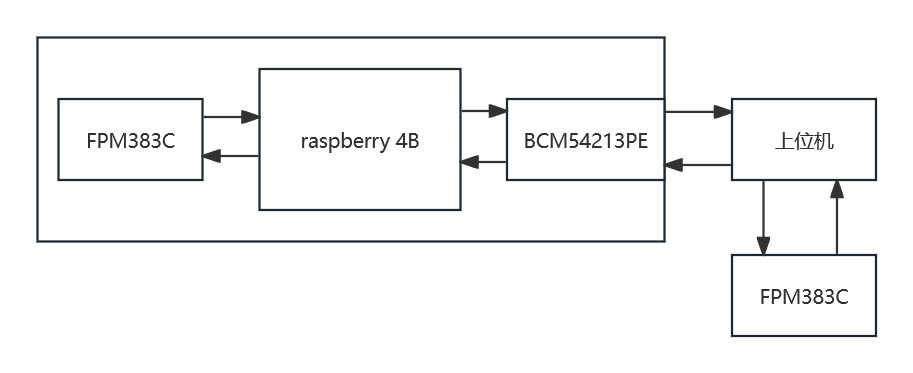
\includegraphics[width=\textwidth]{imgs/总体设计图.png}
    \caption{总体设计图}    \label{overall_design}
\end{figure}

\subsubsection{中央处理芯片选型}

树莓派4B使用的 bcm2711 是一种四核心64位ARM Cortex-A72架构CPU,主频高,能满足多种复杂计算需求以及满足大型程序运行需求。
树莓派4B还存在丰富而完善的接口,两个USb3.0接口,两个USB2.0接口,一个千兆网卡接口,一个HDMI接口,一个CSI接口和一个DSI接口,能够满足对于各种外设的连接需求。
树莓派4B还是树莓派第一个支持不通过 usb 直接访问网卡芯片实现网卡介入的开发板,这无形之中对于实现网卡驱动提供了很多帮助。

\subsubsection{指纹识别模块选型}
FPM383F识别指纹模块功耗低半导体面阵传感器是一款低功耗的光学指纹识别模块,支持对于60组光学指纹进行存储,其通过串口与中央处理器进行通信,在串口驱动方面,使用我开发的 arm\_gpio 库应当开发难度不难。

\subsubsection{通信模块选型}

基于一般企事业单位对于考勤签到需求的需求,我计划提供多种不同的通信模块实现方便选用单位进行选择,其中传统基于 CH304 串口转 TTL 通信模块实现的简单串口通信主要适用于仅对于一两台设备进行支持的情况,而基于网卡模块间接通过网络方式拓展下位机数量的方式是主要计划实现的支持。针对于不同的预算管理需求,计划采用两种不同的方式实现网卡驱动,一种是基于 raspberry4B 板载 bcm54213PE 网卡芯片的驱动线,另一种是基于 ENC28J60,一种基于 SPI 连接的外置 10BASE-T 以太网连接模块实现的。

\subsection{硬件设计}

1. 电路1: 
通过指纹或者按钮,经由GPIO或者UART实现的简单环境信号获取模块电路设计

2. 基于GPIO实现的反馈电路,作用于上位机显示打开成功或者指纹识别模块反馈识别成功时无源蜂鸣器的提示

\subsection{软件设计}